\iffalse

These are R code chunks wrapped in the LaTex markup language. It is woven by the kintr package and typeset into PDF using pdfLaTex. The local installation of LaTex is MikTex 2.9. Additionally, for smaller non-R text, PDF preview is done with the help of Texmaker. The latter is a more sensible choice if no R code is embedded that needs dynamic evaluation. With Texmaker, a large number of Tex packages also become available. Finally, some time was saved by caching some code chunck results using the cache feature in knitr as a number of simulation and optimization procedures are quite time-consuming.

While knitr can also work with R Markdown, which is much simpler to learn and creates good results in html, the knitted html is not optimized for printing. The automatic conversion feature that knitr provides to translate R Markdown to LaTex has little user-control and, especially with graphics, can create the problem of floating in unexpected places.

As such, this file before compiling can also be used to illustrate some basic features of LaTex such as the following

% font size setting
% font change
% margin size change
% table of contents generation
% setting title and subsections
% generating lists and embedded lists
% creating a box frame
% using italics and bold faced letters
% using the math mode, including super- and subscripts, Greek letters, etc.
% adding blank space

\fi


\documentclass[10pt]{article}\usepackage[]{graphicx}\usepackage[]{color}
%% maxwidth is the original width if it is less than linewidth
%% otherwise use linewidth (to make sure the graphics do not exceed the margin)
\makeatletter
\def\maxwidth{ %
  \ifdim\Gin@nat@width>\linewidth
    \linewidth
  \else
    \Gin@nat@width
  \fi
}
\makeatother

\definecolor{fgcolor}{rgb}{0.345, 0.345, 0.345}
\newcommand{\hlnum}[1]{\textcolor[rgb]{0.686,0.059,0.569}{#1}}%
\newcommand{\hlstr}[1]{\textcolor[rgb]{0.192,0.494,0.8}{#1}}%
\newcommand{\hlcom}[1]{\textcolor[rgb]{0.678,0.584,0.686}{\textit{#1}}}%
\newcommand{\hlopt}[1]{\textcolor[rgb]{0,0,0}{#1}}%
\newcommand{\hlstd}[1]{\textcolor[rgb]{0.345,0.345,0.345}{#1}}%
\newcommand{\hlkwa}[1]{\textcolor[rgb]{0.161,0.373,0.58}{\textbf{#1}}}%
\newcommand{\hlkwb}[1]{\textcolor[rgb]{0.69,0.353,0.396}{#1}}%
\newcommand{\hlkwc}[1]{\textcolor[rgb]{0.333,0.667,0.333}{#1}}%
\newcommand{\hlkwd}[1]{\textcolor[rgb]{0.737,0.353,0.396}{\textbf{#1}}}%

\usepackage{framed}
\makeatletter
\newenvironment{kframe}{%
 \def\at@end@of@kframe{}%
 \ifinner\ifhmode%
  \def\at@end@of@kframe{\end{minipage}}%
  \begin{minipage}{\columnwidth}%
 \fi\fi%
 \def\FrameCommand##1{\hskip\@totalleftmargin \hskip-\fboxsep
 \colorbox{shadecolor}{##1}\hskip-\fboxsep
     % There is no \\@totalrightmargin, so:
     \hskip-\linewidth \hskip-\@totalleftmargin \hskip\columnwidth}%
 \MakeFramed {\advance\hsize-\width
   \@totalleftmargin\z@ \linewidth\hsize
   \@setminipage}}%
 {\par\unskip\endMakeFramed%
 \at@end@of@kframe}
\makeatother

\definecolor{shadecolor}{rgb}{.97, .97, .97}
\definecolor{messagecolor}{rgb}{0, 0, 0}
\definecolor{warningcolor}{rgb}{1, 0, 1}
\definecolor{errorcolor}{rgb}{1, 0, 0}
\newenvironment{knitrout}{}{} % an empty environment to be redefined in TeX

\usepackage{alltt}

\addtolength{\oddsidemargin}{-.875in}
\addtolength{\evensidemargin}{-.875in}
\addtolength{\textwidth}{1.75in}
\addtolength{\topmargin}{-.9in}
\addtolength{\textheight}{1.8in}
\IfFileExists{upquote.sty}{\usepackage{upquote}}{}

\begin{document}

\tableofcontents

\title{Basics in Exploratory Data Analysis Using R}
\date{}
\maketitle

This is a simple tutorial introducing some of the basic packages and the useful functions they contain. These tools have wide-ranging applicability and can be easily adapted to financial modeling and risk management purposes.

We will roughly follow the order of topics outlined below.\\

\fbox{
\parbox{15cm}{%
\begin{enumerate}
\item First, we learn to simulate some price processes
\item Then, we try to find ways to fit models to the processes we just went through
\item Finally, we try to make predictions or inferences from the work above
\end{enumerate}}
}
\vspace{5mm}

The packages used in this tutorial are as follows:  
\begin{itemize}
\item sde (stochastic differential equations)  
\item lubridate (for massaging dates)  
\item fGarch (for fitting Garch models)  
\item xlsx (for importing Excel files)  
\item evir (for working with Extreme Value distributions and plots)  
\item ggplot2 (for creating some pretty charts)  
\item mvtnorm (for multivariate normal)  
\item MASS (for fitting some common distributions)  
\item copula (for fitting copulas)  
\item gtools (used here for applying functions to running windows of data)  
\item tseries (for using functions/tests associated with time series)  
\item forecast (for forecasting)  
\item boot (for bootstraping)  
\end{itemize}

\section{Price processes}  

We simulate 100 paths of each of the processes described below, plot them on a chart and show the 5th and 95th percentiles.

\subsection{Random Walk}
$$log(S_{t+\Delta t})=log(S_t)+\mu \Delta t+\sigma \sqrt{\Delta t}Z_t$$
\begin{knitrout}
\definecolor{shadecolor}{rgb}{0.969, 0.969, 0.969}\color{fgcolor}\begin{kframe}
\begin{alltt}
\hlcom{# Model:}
\hlcom{# s     =log(S)}
\hlcom{# r     =diff(s)}
\hlcom{# mu    =mean(r)}
\hlcom{# sigma =std(r)}
\hlcom{# z     =(r-mu)/sigma}
\hlstd{s_0}\hlkwb{=}\hlnum{10}
\hlstd{mu}\hlkwb{=}\hlnum{0.05}\hlopt{/}\hlnum{250}
\hlstd{sigma}\hlkwb{=}\hlnum{0.2}\hlopt{/}\hlkwd{sqrt}\hlstd{(}\hlnum{250}\hlstd{)}
\hlkwd{set.seed}\hlstd{(}\hlnum{123}\hlstd{)}
\hlstd{x}\hlkwb{=}\hlkwd{matrix}\hlstd{(s_0,}\hlkwc{ncol}\hlstd{=}\hlnum{100}\hlstd{,}\hlkwc{nrow}\hlstd{=}\hlnum{10}\hlopt{^}\hlnum{3}\hlstd{)}    \hlcom{#store the 100 bm's in a matrix for plotting}
\hlkwa{for} \hlstd{(t} \hlkwa{in} \hlnum{2}\hlopt{:} \hlnum{10}\hlopt{^}\hlnum{3}\hlstd{)}                  \hlcom{#note how loop is done in R}
  \hlstd{x[t,]}\hlkwb{=}\hlstd{x[t}\hlopt{-}\hlnum{1}\hlstd{,]}\hlopt{+}\hlkwd{rnorm}\hlstd{(}\hlnum{100}\hlstd{)}\hlopt{*}\hlstd{sigma}\hlopt{+}\hlstd{mu} \hlcom{#note the subsetting syntax in R}
\hlkwd{plot}\hlstd{(}\hlkwd{seq}\hlstd{(}\hlnum{0}\hlstd{,}\hlnum{1}\hlstd{,}\hlkwc{le}\hlstd{=}\hlnum{1000}\hlstd{),x[,}\hlnum{1}\hlstd{],}\hlstr{"n"}\hlstd{,}    \hlcom{#note the syntax of the plotting function}
     \hlkwc{ylim}\hlstd{=}\hlkwd{range}\hlstd{(x),}\hlkwc{xlab}\hlstd{=}\hlstr{""}\hlstd{,}\hlkwc{ylab}\hlstd{=}\hlstr{""}\hlstd{)}    \hlcom{#note the beginning of the string in function call}
\hlkwd{polygon}\hlstd{(}\hlkwd{c}\hlstd{(}\hlnum{1}\hlopt{:}\hlnum{10}\hlopt{^}\hlnum{3}\hlstd{,}\hlnum{10}\hlopt{^}\hlnum{3}\hlopt{:}\hlnum{1}\hlstd{)}\hlopt{/}\hlnum{10}\hlopt{^}\hlnum{3}\hlstd{,}\hlkwd{c}\hlstd{(}\hlkwd{apply}\hlstd{(x,}\hlnum{1}\hlstd{,max),}
                                \hlkwd{rev}\hlstd{(}\hlkwd{apply}\hlstd{(x,}\hlnum{1}\hlstd{,min))),}\hlkwc{col}\hlstd{=}\hlstr{"gold"}\hlstd{,}\hlkwc{bor}\hlstd{=F)}
\hlkwd{polygon}\hlstd{(}\hlkwd{c}\hlstd{(}\hlnum{1}\hlopt{:}\hlnum{10}\hlopt{^}\hlnum{3}\hlstd{,}\hlnum{10}\hlopt{^}\hlnum{3}\hlopt{:}\hlnum{1}\hlstd{)}\hlopt{/}\hlnum{10}\hlopt{^}\hlnum{3}\hlstd{,}\hlkwd{c}\hlstd{(}\hlkwd{apply}\hlstd{(x,}\hlnum{1}\hlstd{,quantile,}\hlnum{.95}\hlstd{),}
                                \hlkwd{rev}\hlstd{(}\hlkwd{apply}\hlstd{(x,}\hlnum{1}\hlstd{,quantile,}\hlnum{.05}\hlstd{))),}\hlkwc{col}\hlstd{=}\hlstr{"brown"}\hlstd{,}\hlkwc{bor}\hlstd{=F)}
\end{alltt}
\end{kframe}

{\centering 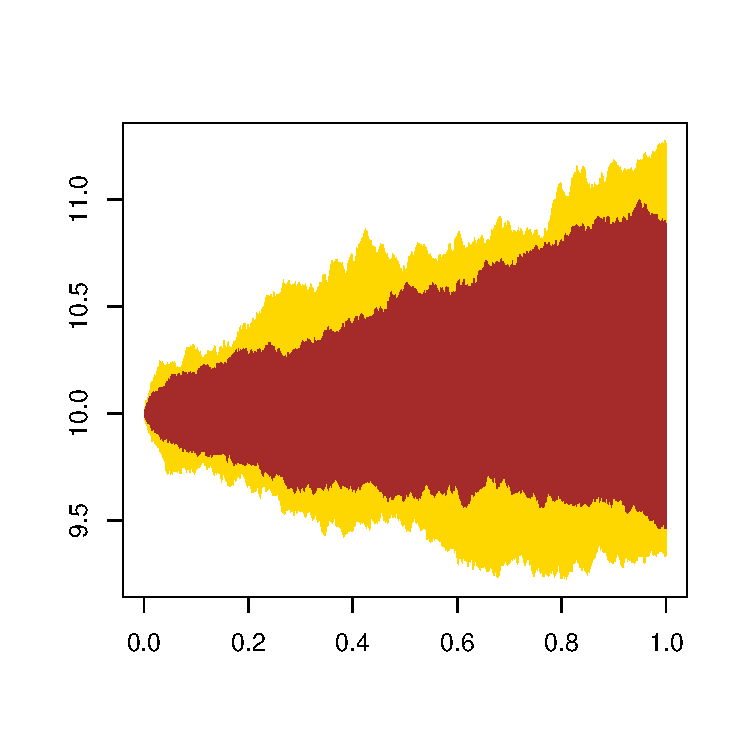
\includegraphics[width=\maxwidth]{figure/unnamed-chunk-1} 

}



\end{knitrout}


\subsection{Mean-Reverting Ornstein-Uhlenbeck Process}
$$dX_t=(\theta_1-\theta_2) dt+\theta_3 dW_t$$
\begin{knitrout}
\definecolor{shadecolor}{rgb}{0.969, 0.969, 0.969}\color{fgcolor}\begin{kframe}
\begin{alltt}
\hlcom{# Model: dXt=(theta1-theta2)*dt+theta3*dWt}
\hlkwd{require}\hlstd{(sde)}
\hlstd{d_OU} \hlkwb{=} \hlkwd{expression}\hlstd{(}\hlopt{-}\hlnum{5} \hlopt{*} \hlstd{x)}
\hlstd{s_OU} \hlkwb{=} \hlkwd{expression}\hlstd{(}\hlnum{3.5}\hlstd{)}
\hlstd{x_OU} \hlkwb{=} \hlkwd{matrix}\hlstd{(s_0,} \hlkwc{ncol} \hlstd{=} \hlnum{100}\hlstd{,} \hlkwc{nrow} \hlstd{=} \hlnum{10}\hlopt{^}\hlnum{3}\hlstd{)}
\hlstd{x_OU} \hlkwb{=} \hlkwd{sde.sim}\hlstd{(}\hlkwc{X0} \hlstd{= s_0,} \hlkwc{drift} \hlstd{= d_OU,} \hlkwc{sigma} \hlstd{= s_OU,} \hlkwc{N} \hlstd{=} \hlnum{999}\hlstd{,} \hlkwc{M} \hlstd{=} \hlnum{100}\hlstd{)}  \hlcom{#N is # of simulation steps}
\hlcom{# M is # of paths}
\hlkwd{plot}\hlstd{(}\hlkwd{seq}\hlstd{(}\hlnum{0}\hlstd{,} \hlnum{1}\hlstd{,} \hlkwc{le} \hlstd{=} \hlnum{1000}\hlstd{), x_OU[,} \hlnum{1}\hlstd{],} \hlstr{"n"}\hlstd{,} \hlkwc{ylim} \hlstd{=} \hlkwd{range}\hlstd{(x_OU),} \hlkwc{xlab} \hlstd{=} \hlstr{""}\hlstd{,} \hlkwc{ylab} \hlstd{=} \hlstr{""}\hlstd{)}
\hlkwd{polygon}\hlstd{(}\hlkwd{c}\hlstd{(}\hlnum{1}\hlopt{:}\hlnum{10}\hlopt{^}\hlnum{3}\hlstd{,} \hlnum{10}\hlopt{^}\hlnum{3}\hlopt{:}\hlnum{1}\hlstd{)}\hlopt{/}\hlnum{10}\hlopt{^}\hlnum{3}\hlstd{,} \hlkwd{c}\hlstd{(}\hlkwd{apply}\hlstd{(x_OU,} \hlnum{1}\hlstd{, max),} \hlkwd{rev}\hlstd{(}\hlkwd{apply}\hlstd{(x_OU,} \hlnum{1}\hlstd{, min))),}
    \hlkwc{col} \hlstd{=} \hlstr{"gold"}\hlstd{,} \hlkwc{bor} \hlstd{= F)}
\hlkwd{polygon}\hlstd{(}\hlkwd{c}\hlstd{(}\hlnum{1}\hlopt{:}\hlnum{10}\hlopt{^}\hlnum{3}\hlstd{,} \hlnum{10}\hlopt{^}\hlnum{3}\hlopt{:}\hlnum{1}\hlstd{)}\hlopt{/}\hlnum{10}\hlopt{^}\hlnum{3}\hlstd{,} \hlkwd{c}\hlstd{(}\hlkwd{apply}\hlstd{(x_OU,} \hlnum{1}\hlstd{, quantile,} \hlnum{0.95}\hlstd{),} \hlkwd{rev}\hlstd{(}\hlkwd{apply}\hlstd{(x_OU,}
    \hlnum{1}\hlstd{, quantile,} \hlnum{0.05}\hlstd{))),} \hlkwc{col} \hlstd{=} \hlstr{"brown"}\hlstd{,} \hlkwc{bor} \hlstd{= F)}
\end{alltt}
\end{kframe}

{\centering 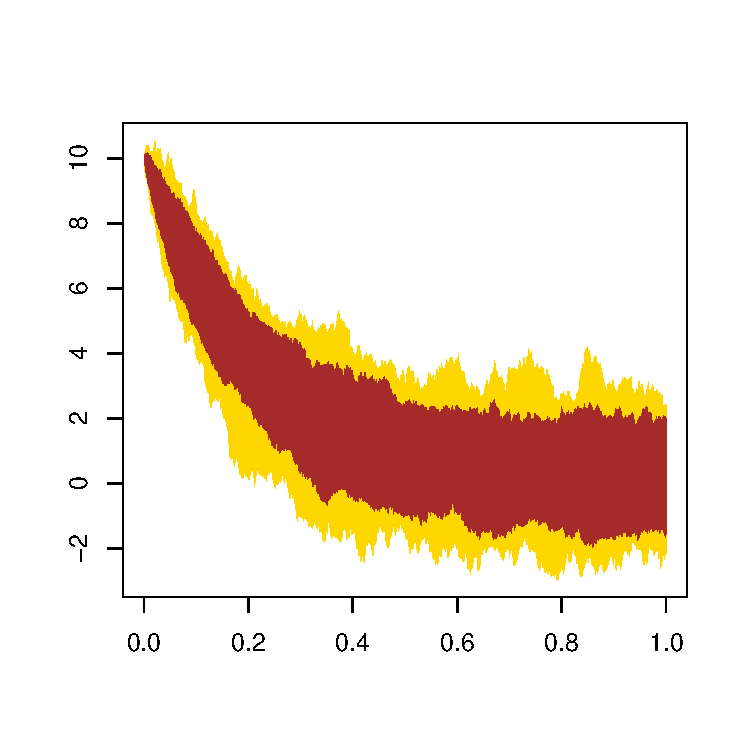
\includegraphics[width=\maxwidth]{figure/unnamed-chunk-2} 

}



\end{knitrout}


\subsection{Cox-Ingersoll-Ross (CIR) Process}  
$$dX_t=(\theta_1-\theta_2) dt+\theta_3 \sqrt{X_t} dW_t$$
\begin{knitrout}
\definecolor{shadecolor}{rgb}{0.969, 0.969, 0.969}\color{fgcolor}\begin{kframe}
\begin{alltt}
\hlcom{# Model: dXt=(theta1-theta2)*dt+theta3*sqrt(Xt)*dWt}
\hlstd{d_CIR} \hlkwb{=} \hlkwd{expression}\hlstd{(}\hlnum{6} \hlopt{-} \hlnum{3} \hlopt{*} \hlstd{x)}
\hlstd{s_CIR} \hlkwb{=} \hlkwd{expression}\hlstd{(}\hlnum{2} \hlopt{*} \hlkwd{sqrt}\hlstd{(x))}
\hlstd{x_CIR} \hlkwb{=} \hlkwd{matrix}\hlstd{(s_0,} \hlkwc{ncol} \hlstd{=} \hlnum{100}\hlstd{,} \hlkwc{nrow} \hlstd{=} \hlnum{10}\hlopt{^}\hlnum{3}\hlstd{)}
\hlstd{x_CIR} \hlkwb{=} \hlkwd{sde.sim}\hlstd{(}\hlkwc{X0} \hlstd{= s_0,} \hlkwc{drift} \hlstd{= d_CIR,} \hlkwc{sigma} \hlstd{= s_CIR,} \hlkwc{N} \hlstd{=} \hlnum{999}\hlstd{,} \hlkwc{M} \hlstd{=} \hlnum{100}\hlstd{)}
\hlkwd{plot}\hlstd{(}\hlkwd{seq}\hlstd{(}\hlnum{0}\hlstd{,} \hlnum{1}\hlstd{,} \hlkwc{le} \hlstd{=} \hlnum{1000}\hlstd{), x_CIR[,} \hlnum{1}\hlstd{],} \hlstr{"n"}\hlstd{,} \hlkwc{ylim} \hlstd{=} \hlkwd{range}\hlstd{(x_CIR),} \hlkwc{xlab} \hlstd{=} \hlstr{""}\hlstd{,}
    \hlkwc{ylab} \hlstd{=} \hlstr{""}\hlstd{)}
\hlkwd{polygon}\hlstd{(}\hlkwd{c}\hlstd{(}\hlnum{1}\hlopt{:}\hlnum{10}\hlopt{^}\hlnum{3}\hlstd{,} \hlnum{10}\hlopt{^}\hlnum{3}\hlopt{:}\hlnum{1}\hlstd{)}\hlopt{/}\hlnum{10}\hlopt{^}\hlnum{3}\hlstd{,} \hlkwd{c}\hlstd{(}\hlkwd{apply}\hlstd{(x_CIR,} \hlnum{1}\hlstd{, max),} \hlkwd{rev}\hlstd{(}\hlkwd{apply}\hlstd{(x_CIR,} \hlnum{1}\hlstd{,}
    \hlstd{min))),} \hlkwc{col} \hlstd{=} \hlstr{"gold"}\hlstd{,} \hlkwc{bor} \hlstd{= F)}
\hlkwd{polygon}\hlstd{(}\hlkwd{c}\hlstd{(}\hlnum{1}\hlopt{:}\hlnum{10}\hlopt{^}\hlnum{3}\hlstd{,} \hlnum{10}\hlopt{^}\hlnum{3}\hlopt{:}\hlnum{1}\hlstd{)}\hlopt{/}\hlnum{10}\hlopt{^}\hlnum{3}\hlstd{,} \hlkwd{c}\hlstd{(}\hlkwd{apply}\hlstd{(x_CIR,} \hlnum{1}\hlstd{, quantile,} \hlnum{0.95}\hlstd{),} \hlkwd{rev}\hlstd{(}\hlkwd{apply}\hlstd{(x_CIR,}
    \hlnum{1}\hlstd{, quantile,} \hlnum{0.05}\hlstd{))),} \hlkwc{col} \hlstd{=} \hlstr{"brown"}\hlstd{,} \hlkwc{bor} \hlstd{= F)}
\end{alltt}
\end{kframe}

{\centering 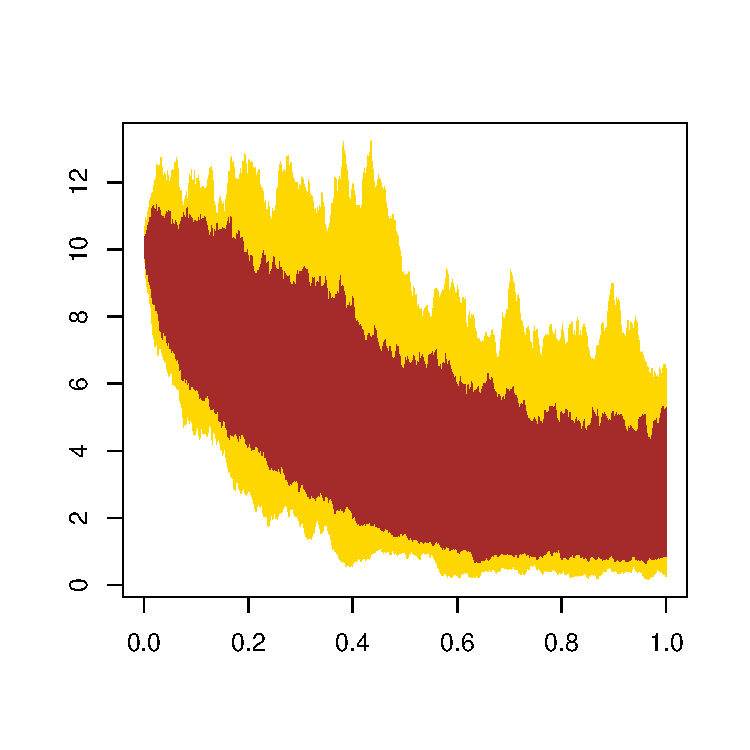
\includegraphics[width=\maxwidth]{figure/unnamed-chunk-3} 

}



\end{knitrout}


\section{Fitting Models} 

\subsection{Some Exploratory Data Analysis}

We plot the histogram of the historical Henry Hub returns data and compare it to that of a normal distribution  

\begin{knitrout}
\definecolor{shadecolor}{rgb}{0.969, 0.969, 0.969}\color{fgcolor}\begin{kframe}
\begin{alltt}
\hlkwd{require}\hlstd{(xlsx)}
\hlstd{histRet} \hlkwb{=} \hlkwd{read.xlsx}\hlstd{(}\hlstr{"C:\textbackslash{}\textbackslash{}Users\textbackslash{}\textbackslash{}Yangster\textbackslash{}\textbackslash{}Dropbox\textbackslash{}\textbackslash{}Private\textbackslash{}\textbackslash{}HistPowerGasSpot_Values2.xlsx"}\hlstd{,}
    \hlnum{1}\hlstd{)}
\hlstd{retHH} \hlkwb{=} \hlstd{histRet[}\hlkwd{which}\hlstd{(histRet}\hlopt{$}\hlstd{Hub} \hlopt{==} \hlstr{"HH"}\hlstd{), ]}

\hlkwd{attach}\hlstd{(retHH)}
\hlkwd{require}\hlstd{(lubridate)}  \hlcom{#Lubridate is a useful dates package }
\hlstd{idx.remove} \hlkwb{=} \hlkwd{which}\hlstd{(Price} \hlopt{==} \hlnum{0}\hlstd{)}  \hlcom{#Clean up HH prices/returns for non-trading days}
\hlstd{retHH} \hlkwb{=} \hlstd{retHH[}\hlopt{-}\hlstd{idx.remove, ]}

\hlstd{y} \hlkwb{=} \hlkwd{ymd}\hlstd{(}\hlkwd{as.character}\hlstd{(Date))}
\hlkwd{par}\hlstd{(}\hlkwc{mar} \hlstd{=} \hlkwd{c}\hlstd{(}\hlnum{4}\hlstd{,} \hlnum{5}\hlstd{,} \hlnum{4}\hlstd{,} \hlnum{2}\hlstd{))}  \hlcom{#Note how to set margins of the plotting device}
\hlkwd{plot}\hlstd{(y, Price,} \hlstr{"l"}\hlstd{,} \hlkwc{xlab} \hlstd{=} \hlstr{"Date"}\hlstd{,} \hlkwc{ylab} \hlstd{=} \hlstr{"Returns"}\hlstd{,} \hlkwc{main} \hlstd{=} \hlstr{"Henry Hub Historical Returns"}\hlstd{)}
\end{alltt}
\end{kframe}

{\centering 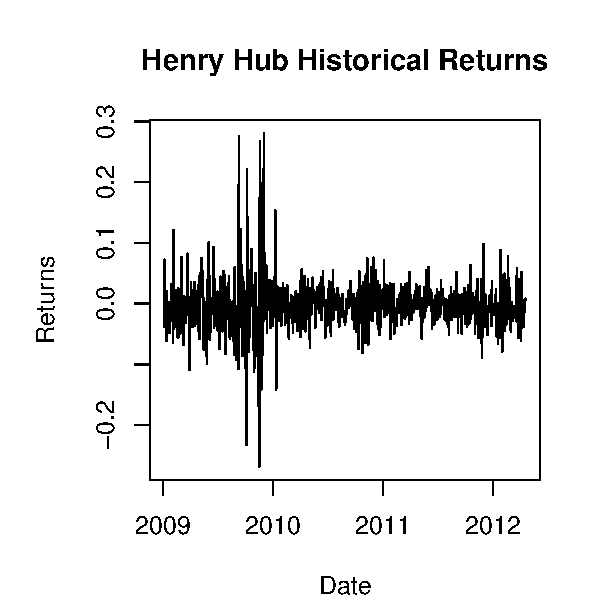
\includegraphics[width=\maxwidth]{figure/unnamed-chunk-41} 

}


\begin{kframe}\begin{alltt}
\hlkwd{hist}\hlstd{(Price,} \hlkwc{breaks} \hlstd{=} \hlnum{30}\hlstd{,} \hlkwc{xlim} \hlstd{=} \hlkwd{range}\hlstd{(Price),} \hlkwc{main} \hlstd{=} \hlstr{"Histogram of HH Returns"}\hlstd{)}
\hlkwd{set.seed}\hlstd{(}\hlnum{123}\hlstd{)}
\hlstd{pSim} \hlkwb{=} \hlkwd{rnorm}\hlstd{(}\hlkwd{length}\hlstd{(Price),} \hlkwc{mean} \hlstd{=} \hlkwd{mean}\hlstd{(Price),} \hlkwc{sd} \hlstd{=} \hlkwd{sd}\hlstd{(Price))}
\hlkwd{hist}\hlstd{(pSim,} \hlkwc{breaks} \hlstd{=} \hlnum{30}\hlstd{,} \hlkwc{add} \hlstd{= T,} \hlkwc{col} \hlstd{=} \hlstr{"red"}\hlstd{)}
\end{alltt}
\end{kframe}

{\centering 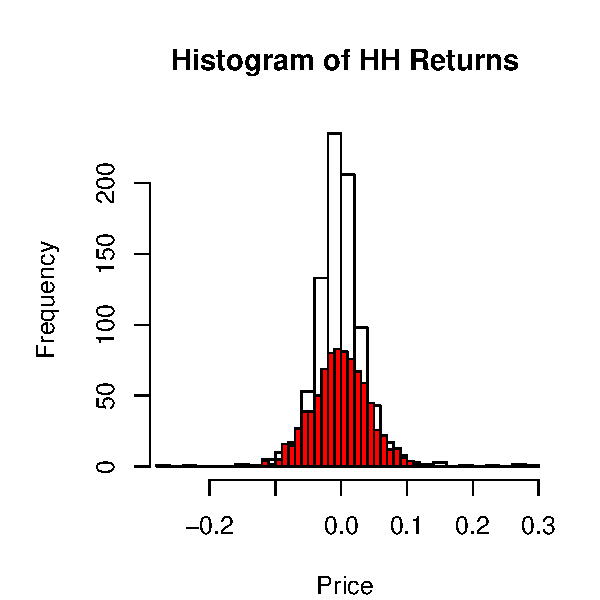
\includegraphics[width=\maxwidth]{figure/unnamed-chunk-42} 

}



\end{knitrout}

Since we are more concerned about the tails of the distribution, we use the functionality of fitting Generalized Pareto Distribution in the \textbf{evir} package and examine the fit of the model with some diagnostic plots.
\begin{knitrout}
\definecolor{shadecolor}{rgb}{0.969, 0.969, 0.969}\color{fgcolor}\begin{kframe}
\begin{alltt}
\hlkwd{require}\hlstd{(evir)}
\hlcom{# Creates a plot showing how the estimate of shape varies with threshold or}
\hlcom{# number of extremes.}
\hlkwd{shape}\hlstd{(Price} \hlopt{* -}\hlnum{1}\hlstd{,} \hlkwc{models} \hlstd{=} \hlnum{30}\hlstd{,} \hlkwc{start} \hlstd{=} \hlnum{15}\hlstd{,} \hlkwc{end} \hlstd{=} \hlnum{100}\hlstd{)}
\end{alltt}
\end{kframe}

{\centering 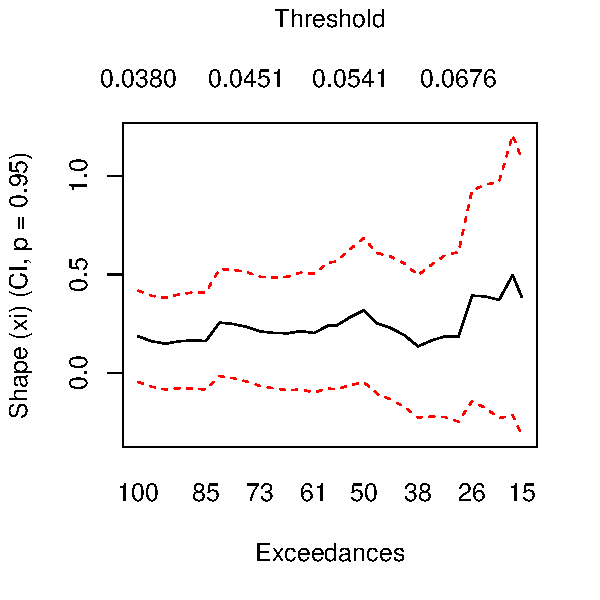
\includegraphics[width=\maxwidth]{figure/unnamed-chunk-51} 

}


\begin{kframe}\begin{alltt}
\hlcom{# Fitting Generalized Pareto Distribution to data}
\hlstd{hh.est} \hlkwb{=} \hlkwd{gpd}\hlstd{(Price} \hlopt{* -}\hlnum{1}\hlstd{,} \hlkwc{nextremes} \hlstd{=} \hlnum{50}\hlstd{)}
\hlkwd{tailplot}\hlstd{(hh.est)}
\end{alltt}
\end{kframe}

{\centering 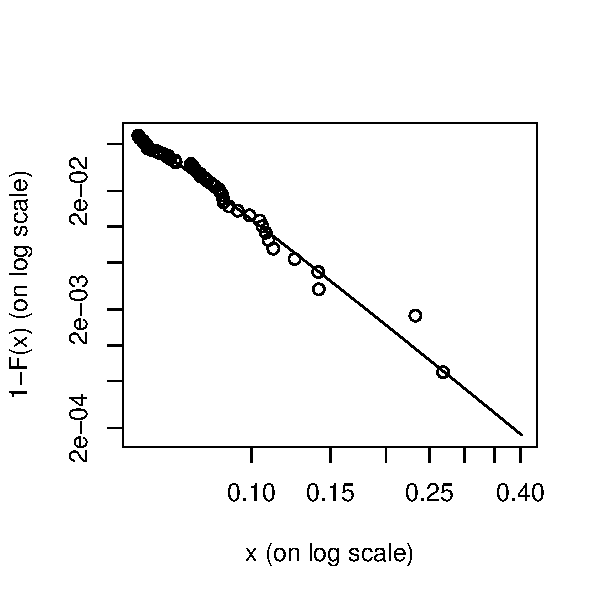
\includegraphics[width=\maxwidth]{figure/unnamed-chunk-52} 

}



\end{knitrout}

Additionally, we can choose from diagnostic graphs created by the command \texttt{plot.gpd()}.
\begin{knitrout}
\definecolor{shadecolor}{rgb}{0.969, 0.969, 0.969}\color{fgcolor}\begin{kframe}
\begin{alltt}
\hlcom{# Simulate from the fitted GPD and compare to the empirical data}
\hlstd{xi.est} \hlkwb{=} \hlstd{hh.est}\hlopt{$}\hlstd{par.ests[}\hlnum{1}\hlstd{]}
\hlstd{beta.est} \hlkwb{=} \hlstd{hh.est}\hlopt{$}\hlstd{par.ests[}\hlnum{2}\hlstd{]}
\hlkwd{hist}\hlstd{(Price,} \hlkwc{breaks} \hlstd{=} \hlnum{30}\hlstd{,} \hlkwc{xlim} \hlstd{=} \hlkwd{range}\hlstd{(Price),} \hlkwc{main} \hlstd{=} \hlstr{"Histogram of HH Returns"}\hlstd{)}
\hlkwd{set.seed}\hlstd{(}\hlnum{123}\hlstd{)}
\hlstd{pSim.gpd} \hlkwb{=} \hlkwd{rgpd}\hlstd{(}\hlkwd{length}\hlstd{(Price),} \hlkwc{xi} \hlstd{= xi.est,} \hlkwc{beta} \hlstd{= beta.est)} \hlopt{* -}\hlnum{1}
\hlkwd{hist}\hlstd{(pSim.gpd,} \hlkwc{breaks} \hlstd{=} \hlnum{30}\hlstd{,} \hlkwc{add} \hlstd{= T)}  \hlcom{#add=T argument overlays the second histogram.}
\end{alltt}
\end{kframe}

{\centering 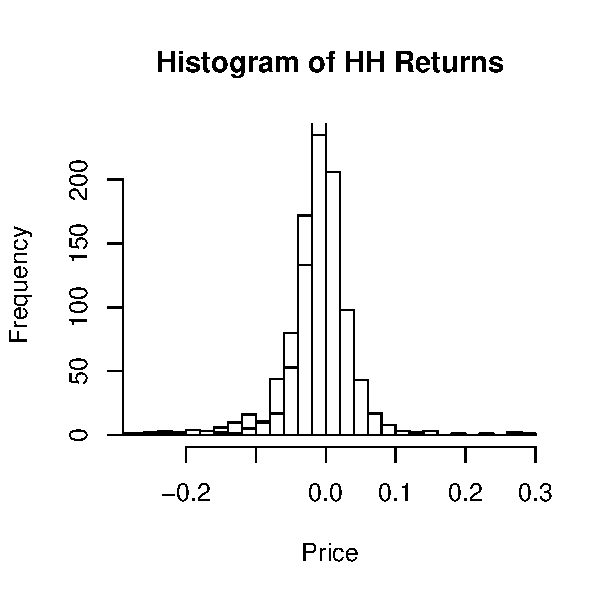
\includegraphics[width=\maxwidth]{figure/unnamed-chunk-6} 

}



\end{knitrout}

The overlay of histograms has become harder to see in the graph above. This prompts us to choose a different plotting method so we have more control over how the output is shown.
\begin{knitrout}
\definecolor{shadecolor}{rgb}{0.969, 0.969, 0.969}\color{fgcolor}\begin{kframe}
\begin{alltt}
\hlcom{# Using the ggplot2 package for visualization}
\hlkwd{require}\hlstd{(ggplot2)}
\hlstd{idx} \hlkwb{=} \hlkwd{c}\hlstd{(}\hlkwd{rep}\hlstd{(}\hlstr{"HH"}\hlstd{,} \hlkwd{length}\hlstd{(Price)),} \hlkwd{rep}\hlstd{(}\hlstr{"GPD"}\hlstd{,} \hlkwd{length}\hlstd{(Price)))}
\hlstd{hist.Comb} \hlkwb{=} \hlkwd{data.frame}\hlstd{(idx,} \hlkwd{c}\hlstd{(Price, pSim.gpd))}
\hlkwd{colnames}\hlstd{(hist.Comb)} \hlkwb{=} \hlkwd{c}\hlstd{(}\hlstr{"Index"}\hlstd{,} \hlstr{"Returns"}\hlstd{)}
\hlkwd{ggplot}\hlstd{(hist.Comb,} \hlkwd{aes}\hlstd{(Returns,} \hlkwc{fill} \hlstd{= Index))} \hlopt{+} \hlkwd{geom_density}\hlstd{(}\hlkwc{alpha} \hlstd{=} \hlnum{0.2}\hlstd{)} \hlopt{+}
    \hlkwd{coord_cartesian}\hlstd{(}\hlkwc{xlim} \hlstd{=} \hlkwd{c}\hlstd{(}\hlopt{-}\hlnum{0}\hlstd{,} \hlopt{-}\hlnum{0.4}\hlstd{),} \hlkwc{ylim} \hlstd{=} \hlkwd{c}\hlstd{(}\hlnum{0}\hlstd{,} \hlnum{5}\hlstd{))}
\end{alltt}
\end{kframe}

{\centering 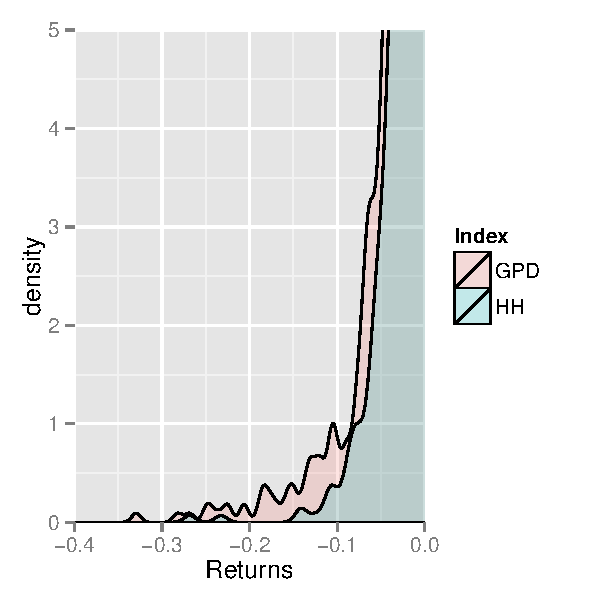
\includegraphics[width=\maxwidth]{figure/unnamed-chunk-7} 

}



\end{knitrout}


\subsection{Fitting a GARCH (1,1) Model}  
\begin{knitrout}
\definecolor{shadecolor}{rgb}{0.969, 0.969, 0.969}\color{fgcolor}\begin{kframe}
\begin{alltt}
\hlkwd{require}\hlstd{(fGarch)}
\hlstd{modGarch} \hlkwb{<-} \hlkwd{garchFit}\hlstd{(}\hlkwc{formula} \hlstd{=} \hlopt{~}\hlkwd{garch}\hlstd{(}\hlnum{1}\hlstd{,} \hlnum{1}\hlstd{),} \hlkwc{data} \hlstd{= Price,} \hlkwc{cond.dist} \hlstd{=} \hlstr{"norm"}\hlstd{)}
\hlkwd{summary}\hlstd{(modGarch)}
\hlkwd{str}\hlstd{(modGarch)}  \hlcom{#To see the structure of the object returned by modGarch for later use}
\hlkwd{set.seed}\hlstd{(}\hlnum{123}\hlstd{)}
\hlstd{parList} \hlkwb{=} \hlstd{modGarch}\hlopt{@}\hlkwc{fit}\hlopt{$}\hlstd{par}
\hlstd{modGarchSpec} \hlkwb{=} \hlkwd{garchSpec}\hlstd{(}\hlkwc{model} \hlstd{= parList,} \hlkwc{cond.dist} \hlstd{=} \hlstr{"norm"}\hlstd{)}
\hlstd{simGarch} \hlkwb{<-} \hlkwd{garchSim}\hlstd{(modGarchSpec,} \hlkwc{n} \hlstd{=} \hlkwd{length}\hlstd{(y))}
\hlkwd{plot}\hlstd{(y, Price,} \hlstr{"l"}\hlstd{,} \hlkwc{xlab} \hlstd{=} \hlstr{"Date"}\hlstd{,} \hlkwc{ylab} \hlstd{=} \hlstr{"Returns"}\hlstd{,} \hlkwc{main} \hlstd{=} \hlstr{"Henry Hub Historical Returns"}\hlstd{)}
\hlkwd{lines}\hlstd{(y, simGarch,} \hlkwc{col} \hlstd{=} \hlstr{"red"}\hlstd{)}
\end{alltt}
\end{kframe}

{\centering 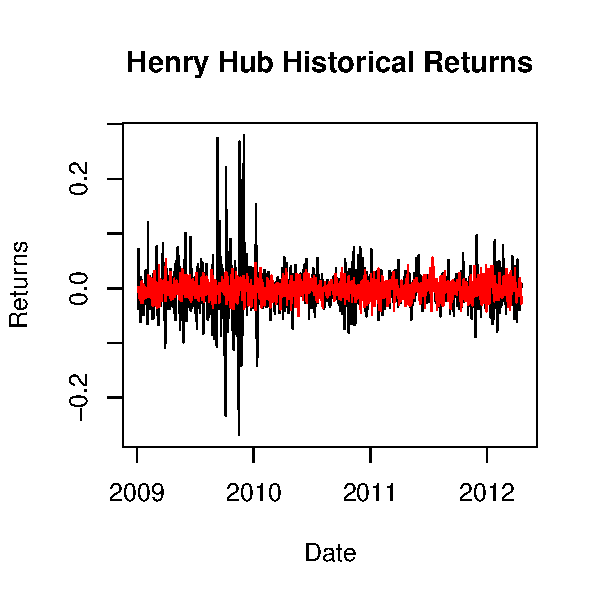
\includegraphics[width=\maxwidth]{figure/unnamed-chunk-8} 

}



\end{knitrout}

The larger swings don't seem to be captured very well in the plot above. Is this because the Garch model is not calibrating to the outlier values in 2009-2010 period? Let's zoom in on a smaller band.

\begin{knitrout}
\definecolor{shadecolor}{rgb}{0.969, 0.969, 0.969}\color{fgcolor}\begin{kframe}
\begin{alltt}
\hlkwd{plot}\hlstd{(y, Price,} \hlstr{"l"}\hlstd{,} \hlkwc{xlab} \hlstd{=} \hlstr{"Date"}\hlstd{,} \hlkwc{ylab} \hlstd{=} \hlstr{"Returns"}\hlstd{,} \hlkwc{main} \hlstd{=} \hlstr{"Henry Hub Historical Returns"}\hlstd{,}
    \hlkwc{ylim} \hlstd{=} \hlkwd{c}\hlstd{(}\hlopt{-}\hlnum{0.1}\hlstd{,} \hlnum{0.1}\hlstd{))}
\hlkwd{lines}\hlstd{(y, simGarch,} \hlkwc{col} \hlstd{=} \hlstr{"red"}\hlstd{)}
\end{alltt}
\end{kframe}

{\centering 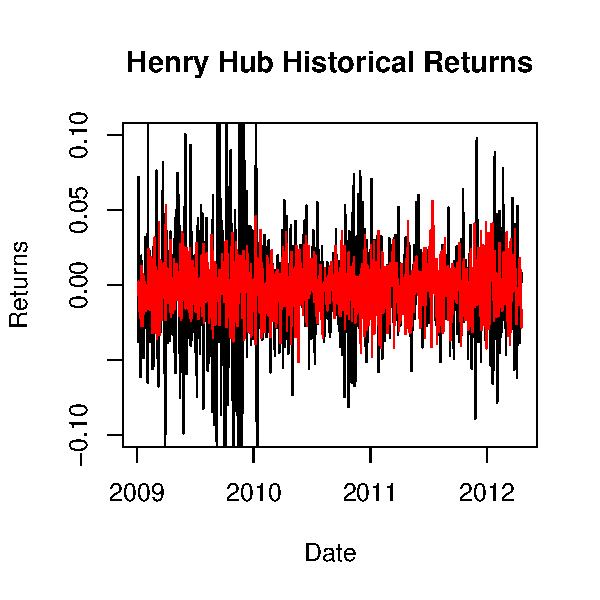
\includegraphics[width=\maxwidth]{figure/unnamed-chunk-91} 

}


\begin{kframe}\begin{alltt}
\hlkwd{predict}\hlstd{(modGarch,} \hlkwc{n.ahead} \hlstd{=} \hlnum{10}\hlstd{,} \hlkwc{plot} \hlstd{=} \hlnum{TRUE}\hlstd{)}
\end{alltt}
\end{kframe}

{\centering 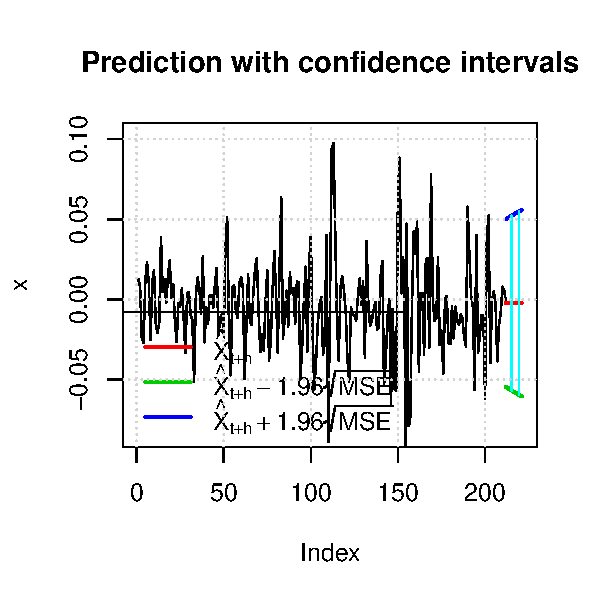
\includegraphics[width=\maxwidth]{figure/unnamed-chunk-92} 

}



\end{knitrout}

We can also plot the 5th and 95th quantiles of the empirical data against the same quantiles of the simulated data using the fitted Garch model to gaugue how well the model performs.
\begin{knitrout}
\definecolor{shadecolor}{rgb}{0.969, 0.969, 0.969}\color{fgcolor}\begin{kframe}
\begin{alltt}
\hlstd{quant} \hlkwb{=} \hlkwd{matrix}\hlstd{(}\hlnum{0}\hlstd{,} \hlkwc{ncol} \hlstd{=} \hlnum{2}\hlstd{,} \hlkwc{nrow} \hlstd{= (}\hlkwd{length}\hlstd{(y)} \hlopt{-} \hlnum{99}\hlstd{))}
\hlstd{quantSim} \hlkwb{=} \hlkwd{matrix}\hlstd{(}\hlnum{0}\hlstd{,} \hlkwc{ncol} \hlstd{=} \hlnum{2}\hlstd{,} \hlkwc{nrow} \hlstd{= (}\hlkwd{length}\hlstd{(y)} \hlopt{-} \hlnum{99}\hlstd{))}
\hlkwa{for} \hlstd{(i} \hlkwa{in} \hlnum{100}\hlopt{:}\hlkwd{length}\hlstd{(y)) \{}
    \hlstd{quant[i} \hlopt{-} \hlnum{99}\hlstd{,} \hlnum{1}\hlstd{]} \hlkwb{=} \hlkwd{quantile}\hlstd{(Price[i} \hlopt{-} \hlnum{99}\hlopt{:}\hlstd{i],} \hlkwc{probs} \hlstd{=} \hlnum{0.05}\hlstd{)}
    \hlstd{quant[i} \hlopt{-} \hlnum{99}\hlstd{,} \hlnum{2}\hlstd{]} \hlkwb{=} \hlkwd{quantile}\hlstd{(Price[i} \hlopt{-} \hlnum{99}\hlopt{:}\hlstd{i],} \hlkwc{probs} \hlstd{=} \hlnum{0.95}\hlstd{)}
\hlstd{\}}

\hlkwd{plot}\hlstd{(y, Price,} \hlstr{"l"}\hlstd{,} \hlkwc{xlab} \hlstd{=} \hlstr{"Date"}\hlstd{,} \hlkwc{ylab} \hlstd{=} \hlstr{"Returns"}\hlstd{,} \hlkwc{main} \hlstd{=} \hlstr{"Henry Hub Historical Returns"}\hlstd{,}
    \hlkwc{ylim} \hlstd{=} \hlkwd{c}\hlstd{(}\hlopt{-}\hlnum{0.1}\hlstd{,} \hlnum{0.1}\hlstd{))}
\hlkwd{lines}\hlstd{(y[}\hlnum{100}\hlopt{:}\hlkwd{length}\hlstd{(y)], quant[,} \hlnum{1}\hlstd{],} \hlkwc{col} \hlstd{=} \hlstr{"red"}\hlstd{,} \hlkwc{ty} \hlstd{=} \hlstr{"l"}\hlstd{,} \hlkwc{lwd} \hlstd{=} \hlnum{3}\hlstd{)}
\hlkwd{lines}\hlstd{(y[}\hlnum{100}\hlopt{:}\hlkwd{length}\hlstd{(y)], quant[,} \hlnum{2}\hlstd{],} \hlkwc{col} \hlstd{=} \hlstr{"red"}\hlstd{,} \hlkwc{ty} \hlstd{=} \hlstr{"l"}\hlstd{,} \hlkwc{lwd} \hlstd{=} \hlnum{3}\hlstd{)}
\hlkwa{for} \hlstd{(i} \hlkwa{in} \hlnum{100}\hlopt{:}\hlkwd{length}\hlstd{(y)) \{}
    \hlstd{quantSim[i} \hlopt{-} \hlnum{99}\hlstd{,} \hlnum{1}\hlstd{]} \hlkwb{=} \hlkwd{quantile}\hlstd{(simGarch[i} \hlopt{-} \hlnum{99}\hlopt{:}\hlstd{i],} \hlkwc{probs} \hlstd{=} \hlnum{0.05}\hlstd{)}
    \hlstd{quantSim[i} \hlopt{-} \hlnum{99}\hlstd{,} \hlnum{2}\hlstd{]} \hlkwb{=} \hlkwd{quantile}\hlstd{(simGarch[i} \hlopt{-} \hlnum{99}\hlopt{:}\hlstd{i],} \hlkwc{probs} \hlstd{=} \hlnum{0.95}\hlstd{)}
\hlstd{\}}
\hlkwd{lines}\hlstd{(y[}\hlnum{100}\hlopt{:}\hlkwd{length}\hlstd{(y)], quantSim[,} \hlnum{1}\hlstd{],} \hlkwc{col} \hlstd{=} \hlstr{"blue"}\hlstd{,} \hlkwc{ty} \hlstd{=} \hlstr{"p"}\hlstd{)}
\hlkwd{lines}\hlstd{(y[}\hlnum{100}\hlopt{:}\hlkwd{length}\hlstd{(y)], quantSim[,} \hlnum{2}\hlstd{],} \hlkwc{col} \hlstd{=} \hlstr{"blue"}\hlstd{,} \hlkwc{ty} \hlstd{=} \hlstr{"p"}\hlstd{)}
\end{alltt}
\end{kframe}

{\centering 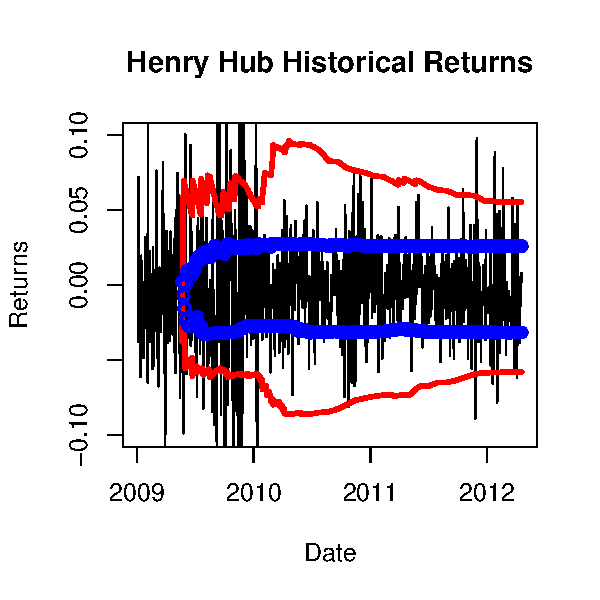
\includegraphics[width=\maxwidth]{figure/unnamed-chunk-10} 

}



\end{knitrout}


\subsection{Analysis of Dependence Structure}  
We begin with some simple plots showing the relationship between WTI and Henry Hub returns. We plot in addition the Q-Q plots for the marginals (WTI and HH) separately, a simulated bivariate normal, and side-by-side plot of the two returns series.
\begin{knitrout}
\definecolor{shadecolor}{rgb}{0.969, 0.969, 0.969}\color{fgcolor}\begin{kframe}
\begin{alltt}
\hlkwd{require}\hlstd{(xlsx)}
\hlstd{histRet2} \hlkwb{=} \hlkwd{read.xlsx}\hlstd{(}\hlstr{"C:\textbackslash{}\textbackslash{}Users\textbackslash{}\textbackslash{}Yangster\textbackslash{}\textbackslash{}Dropbox\textbackslash{}\textbackslash{}Private\textbackslash{}\textbackslash{}HistOilGasSpot.xlsx"}\hlstd{,}
    \hlnum{1}\hlstd{)}
\hlkwd{attach}\hlstd{(histRet2)}
\hlkwd{require}\hlstd{(lubridate)}
\hlstd{y} \hlkwb{=} \hlkwd{ymd}\hlstd{(}\hlkwd{as.character}\hlstd{(Date))}
\hlstd{range_axis} \hlkwb{=} \hlkwd{range}\hlstd{(HH)}
\hlkwd{par}\hlstd{(}\hlkwc{pty} \hlstd{=} \hlstr{"s"}\hlstd{)}
\hlkwd{plot}\hlstd{(HH, WTI,} \hlkwc{xlim} \hlstd{= range_axis,} \hlkwc{ylim} \hlstd{= range_axis,} \hlkwc{main} \hlstd{=} \hlstr{"HH vs. WTI"}\hlstd{)}
\hlkwd{par}\hlstd{(}\hlkwc{pty} \hlstd{=} \hlstr{"m"}\hlstd{)}
\hlstd{mu_2} \hlkwb{=} \hlkwd{c}\hlstd{(}\hlkwd{mean}\hlstd{(HH),} \hlkwd{mean}\hlstd{(WTI))}
\hlstd{sigma_2} \hlkwb{=} \hlkwd{var}\hlstd{(}\hlkwd{cbind}\hlstd{(HH, WTI))}
\hlkwd{require}\hlstd{(mvtnorm)}
\hlstd{simNorm_2} \hlkwb{=} \hlkwd{rmvnorm}\hlstd{(}\hlkwd{length}\hlstd{(HH),} \hlkwc{mean} \hlstd{= mu_2,} \hlkwc{sigma} \hlstd{= sigma_2)}
\hlkwd{par}\hlstd{(}\hlkwc{mfrow} \hlstd{=} \hlkwd{c}\hlstd{(}\hlnum{1}\hlstd{,} \hlnum{2}\hlstd{))}
\hlkwd{plot}\hlstd{(HH, WTI,} \hlkwc{xlim} \hlstd{= range_axis,} \hlkwc{ylim} \hlstd{= range_axis,} \hlkwc{main} \hlstd{=} \hlstr{"HH vs. WTI"}\hlstd{)}
\hlkwd{plot}\hlstd{(simNorm_2,} \hlkwc{xlim} \hlstd{= range_axis,} \hlkwc{ylim} \hlstd{= range_axis,} \hlkwc{main} \hlstd{=} \hlstr{"Simulated Normal"}\hlstd{,}
    \hlkwc{xlab} \hlstd{=} \hlstr{"HH_sim"}\hlstd{,} \hlkwc{ylab} \hlstd{=} \hlstr{"WTI_sim"}\hlstd{)}
\end{alltt}
\end{kframe}

{\centering 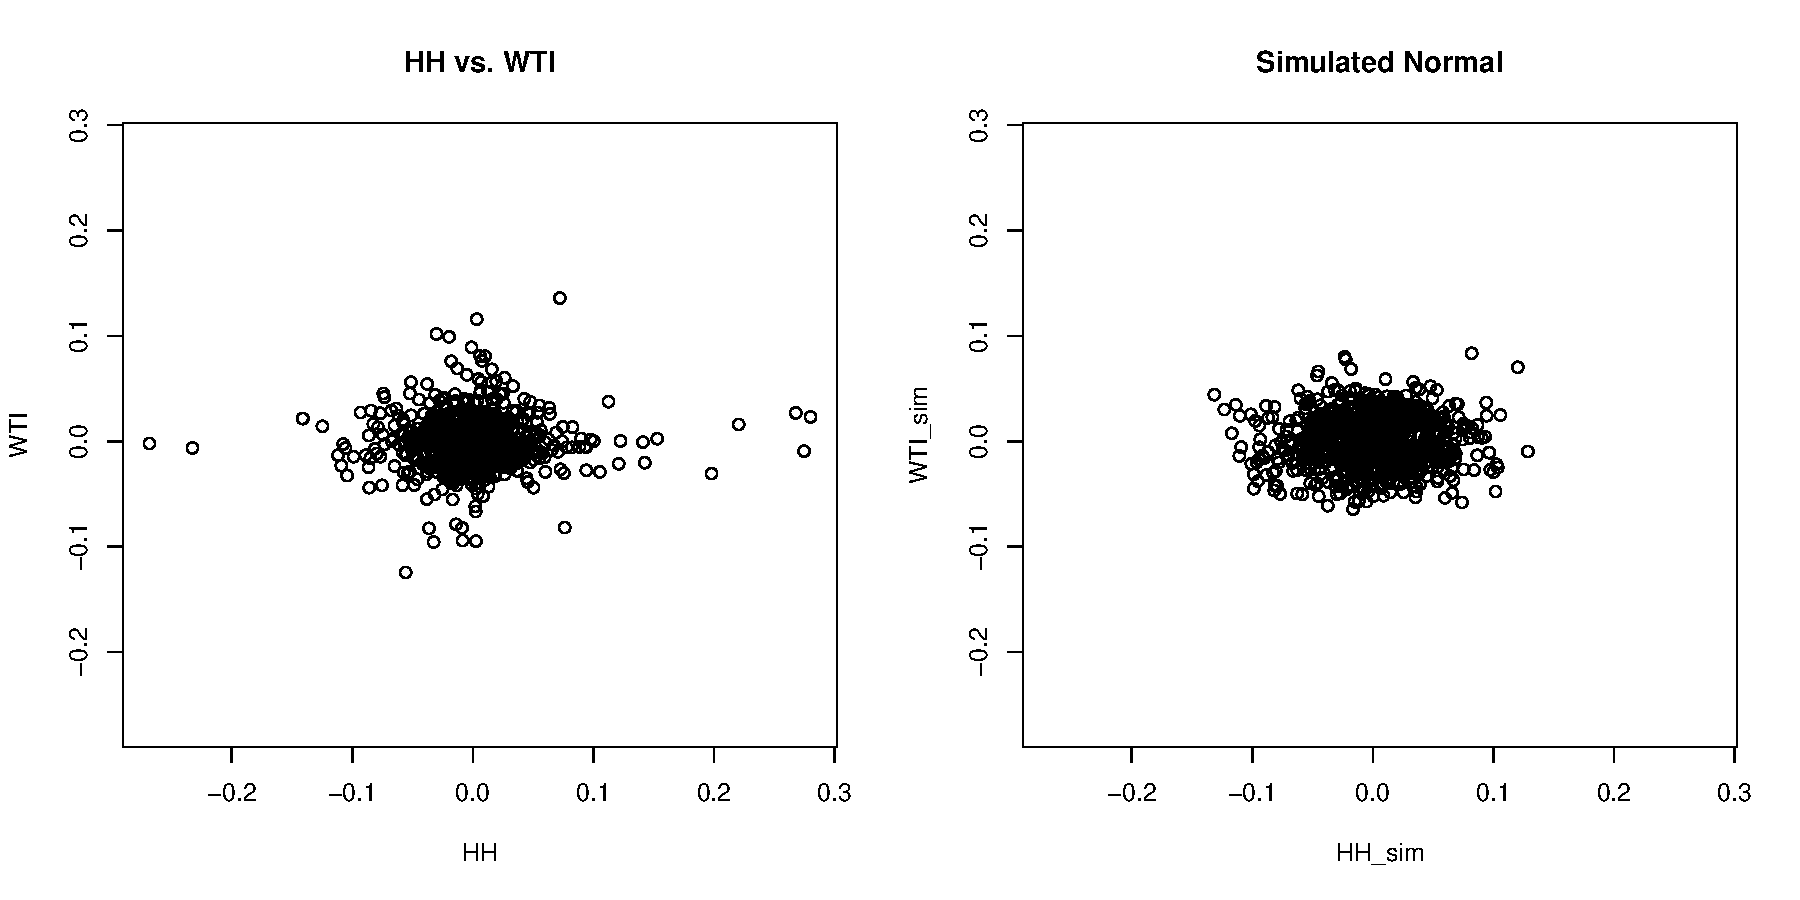
\includegraphics[width=\maxwidth]{figure/unnamed-chunk-111} 

}


\begin{kframe}\begin{alltt}
\hlkwd{qqnorm}\hlstd{(HH,} \hlkwc{main} \hlstd{=} \hlstr{"Q-Q for HH"}\hlstd{)}
\hlkwd{qqnorm}\hlstd{(WTI,} \hlkwc{main} \hlstd{=} \hlstr{"Q-Q for WTI"}\hlstd{)}
\end{alltt}
\end{kframe}

{\centering 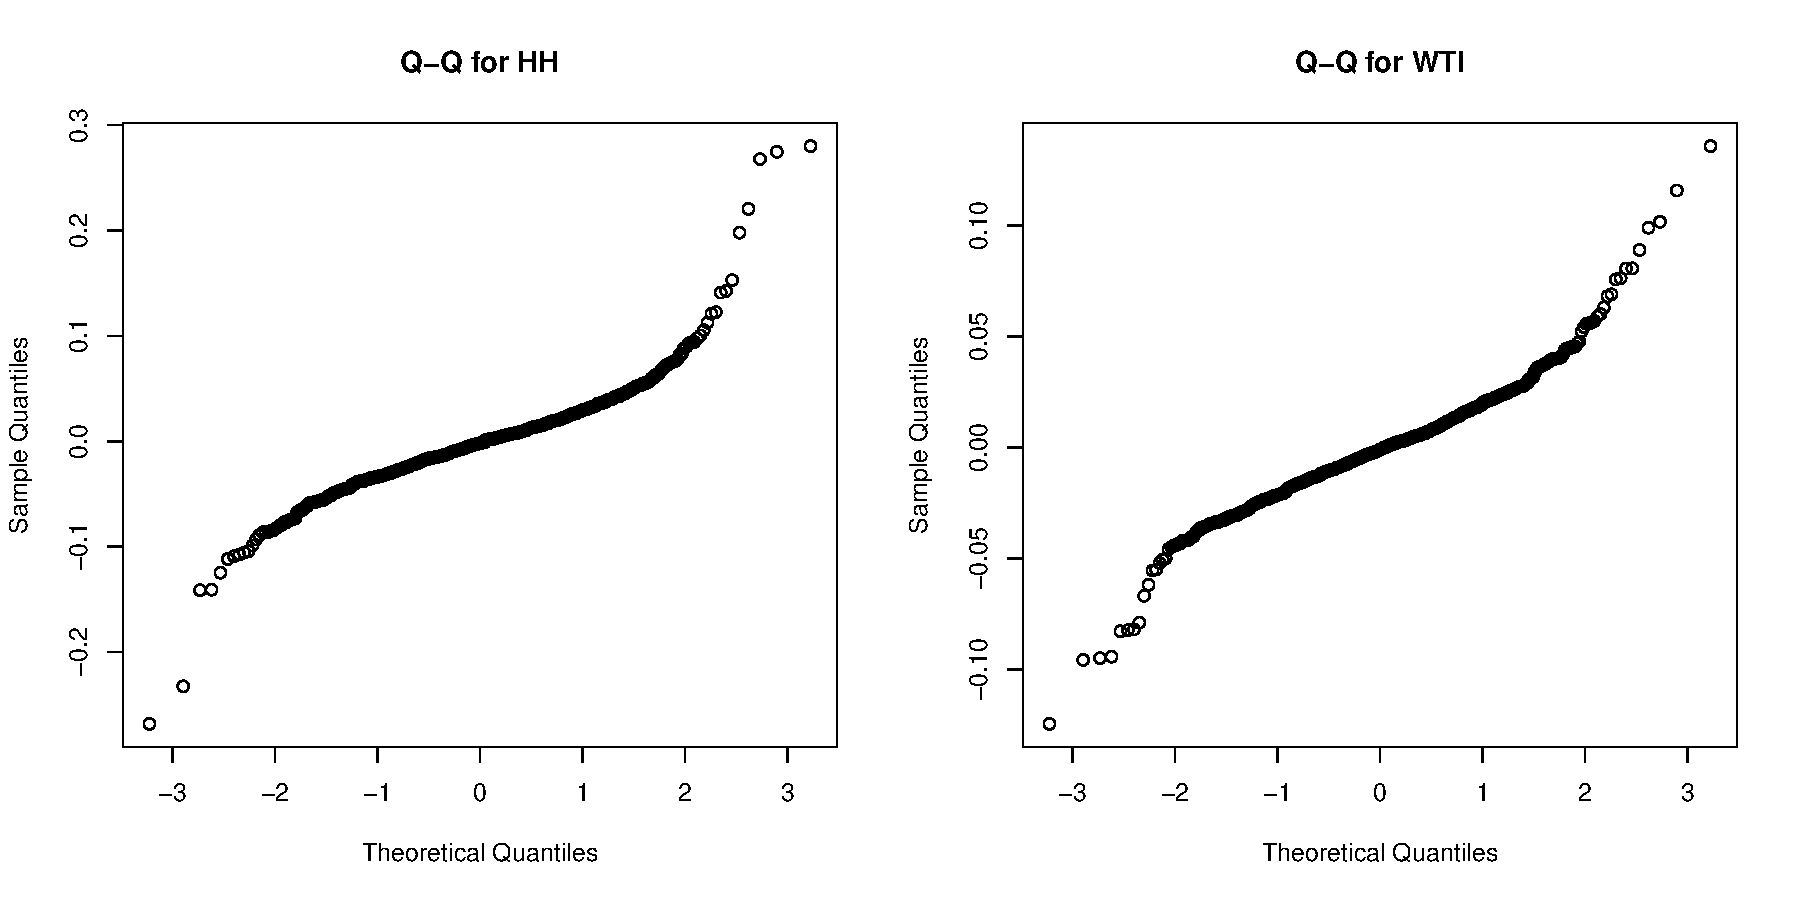
\includegraphics[width=\maxwidth]{figure/unnamed-chunk-112} 

}



\end{knitrout}

\begin{knitrout}
\definecolor{shadecolor}{rgb}{0.969, 0.969, 0.969}\color{fgcolor}\begin{kframe}
\begin{alltt}
\hlcom{# Plot the returns series side by side}
\hlkwd{par}\hlstd{(}\hlkwc{mfrow} \hlstd{=} \hlkwd{c}\hlstd{(}\hlnum{2}\hlstd{,} \hlnum{1}\hlstd{))}
\hlkwd{par}\hlstd{(}\hlkwc{mar} \hlstd{=} \hlkwd{c}\hlstd{(}\hlnum{2}\hlstd{,} \hlnum{2.5}\hlstd{,} \hlnum{2}\hlstd{,} \hlnum{1}\hlstd{))}
\hlkwd{plot}\hlstd{(y, HH,} \hlstr{"l"}\hlstd{,} \hlkwc{main} \hlstd{=} \hlstr{"Henry Hub Historical Returns"}\hlstd{,} \hlkwc{cex.lab} \hlstd{=} \hlnum{0.8}\hlstd{,} \hlkwc{cex.main} \hlstd{=} \hlnum{0.8}\hlstd{,}
    \hlkwc{cex.axis} \hlstd{=} \hlnum{0.8}\hlstd{)}
\hlkwd{plot}\hlstd{(y, WTI,} \hlstr{"l"}\hlstd{,} \hlkwc{main} \hlstd{=} \hlstr{"WTI Historical Returns"}\hlstd{,} \hlkwc{cex.lab} \hlstd{=} \hlnum{0.8}\hlstd{,} \hlkwc{cex.main} \hlstd{=} \hlnum{0.8}\hlstd{,}
    \hlkwc{cex.axis} \hlstd{=} \hlnum{0.8}\hlstd{)}
\end{alltt}
\end{kframe}

{\centering 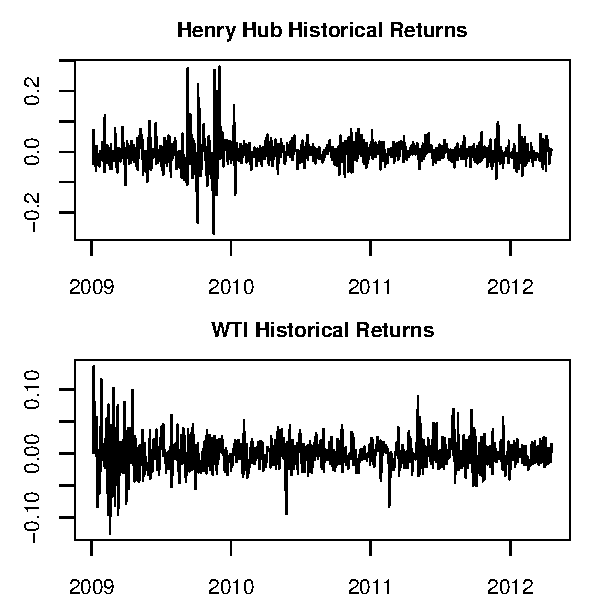
\includegraphics[width=\maxwidth]{figure/unnamed-chunk-12} 

}


\begin{kframe}\begin{alltt}
\hlkwd{par}\hlstd{(}\hlkwc{mfrow} \hlstd{=} \hlkwd{c}\hlstd{(}\hlnum{1}\hlstd{,} \hlnum{1}\hlstd{))}
\hlkwd{par}\hlstd{(}\hlkwc{mar} \hlstd{=} \hlkwd{c}\hlstd{(}\hlnum{4}\hlstd{,} \hlnum{5}\hlstd{,} \hlnum{4}\hlstd{,} \hlnum{2}\hlstd{))}
\end{alltt}
\end{kframe}
\end{knitrout}

Next we look at some measures of dependence.
\begin{knitrout}
\definecolor{shadecolor}{rgb}{0.969, 0.969, 0.969}\color{fgcolor}\begin{kframe}
\begin{alltt}
\hlcom{# Pearson's linear correlation}
\hlkwd{cor}\hlstd{(HH, WTI,} \hlkwc{method} \hlstd{=} \hlstr{"pearson"}\hlstd{)}
\end{alltt}
\begin{verbatim}
## [1] 0.02568
\end{verbatim}
\begin{alltt}
\hlcom{# Kendall's tau}
\hlkwd{cor}\hlstd{(HH, WTI,} \hlkwc{method} \hlstd{=} \hlstr{"kendall"}\hlstd{)}
\end{alltt}
\begin{verbatim}
## [1] 0.005194
\end{verbatim}
\begin{alltt}
\hlcom{# Spearman's rho}
\hlkwd{cor}\hlstd{(HH, WTI,} \hlkwc{method} \hlstd{=} \hlstr{"spearman"}\hlstd{)}
\end{alltt}
\begin{verbatim}
## [1] 0.008645
\end{verbatim}
\end{kframe}
\end{knitrout}

We also look at the distribution for Henry Hub and WTI separately.
\begin{knitrout}
\definecolor{shadecolor}{rgb}{0.969, 0.969, 0.969}\color{fgcolor}\begin{kframe}
\begin{alltt}
\hlcom{# Fit both t and normal distributions to compare loglik}
\hlkwd{require}\hlstd{(}\hlstr{"MASS"}\hlstd{)}
\hlkwd{fitdistr}\hlstd{(HH,} \hlstr{"t"}\hlstd{)}
\end{alltt}
\begin{verbatim}
##        m           s          df    
##   -0.002285    0.026349    3.184829 
##  ( 0.001139) ( 0.001171) ( 0.382361)
\end{verbatim}
\begin{alltt}
\hlkwd{fitdistr}\hlstd{(HH,} \hlstr{"normal"}\hlstd{)}
\end{alltt}
\begin{verbatim}
##      mean         sd    
##   -0.001208    0.042982 
##  ( 0.001525) ( 0.001079)
\end{verbatim}
\begin{alltt}
\hlkwd{fitdistr}\hlstd{(WTI,} \hlstr{"t"}\hlstd{)}
\end{alltt}
\begin{verbatim}
##        m            s            df    
##   -0.0010697    0.0173135    3.8717878 
##  ( 0.0007314) ( 0.0007525) ( 0.5441782)
\end{verbatim}
\begin{alltt}
\hlkwd{fitdistr}\hlstd{(WTI,} \hlstr{"normal"}\hlstd{)}
\end{alltt}
\begin{verbatim}
##       mean          sd    
##   -0.0004216    0.0245263 
##  ( 0.0008704) ( 0.0006155)
\end{verbatim}
\end{kframe}
\end{knitrout}

To fit the full dependence structure, we use the marginal + copula approach (See \textit{Statistics and Data Analysis for Financial Engineering} (P198) for further details).
\begin{enumerate}
\item we fit t distribution to each of the marginals
\item we define a mvdc object (in the \textbf{copula} package)
\item we pass some initial values to an \textit{optim} routine to searh for parameters (the search can fail)  
\end{enumerate}

Before we do so, we briefly mention some classes of copulas commonly encountered in the literature.  

\begin{enumerate}
\item Copula families: Elliptical Copula  
    \begin{enumerate}
    \item Gausssian                       
    \item Student-t
    \end{enumerate}

\item Copula families: Arhimedian Copula  
    \begin{enumerate}
    \item Clayton's Copula                
    \item Gumbel's Copula                 
    \item Frank's Copula
    \end{enumerate}

\item Copula families: Extreme Value Copula  
\end{enumerate}

\begin{knitrout}
\definecolor{shadecolor}{rgb}{0.969, 0.969, 0.969}\color{fgcolor}\begin{kframe}
\begin{alltt}
\hlstd{est.WTI} \hlkwb{=} \hlkwd{as.numeric}\hlstd{(}\hlkwd{fitdistr}\hlstd{(WTI,} \hlstr{"t"}\hlstd{)}\hlopt{$}\hlstd{estimate)}
\hlstd{est.HH} \hlkwb{=} \hlkwd{as.numeric}\hlstd{(}\hlkwd{fitdistr}\hlstd{(HH,} \hlstr{"t"}\hlstd{)}\hlopt{$}\hlstd{estimate)}
\hlcom{# The scale parameter of the fitted t is converted to sd below}
\hlstd{est.WTI[}\hlnum{2}\hlstd{]} \hlkwb{=} \hlstd{est.WTI[}\hlnum{2}\hlstd{]} \hlopt{*} \hlkwd{sqrt}\hlstd{(est.WTI[}\hlnum{3}\hlstd{]}\hlopt{/}\hlstd{(est.WTI[}\hlnum{3}\hlstd{]} \hlopt{-} \hlnum{2}\hlstd{))}
\hlstd{est.HH[}\hlnum{2}\hlstd{]} \hlkwb{=} \hlstd{est.HH[}\hlnum{2}\hlstd{]} \hlopt{*} \hlkwd{sqrt}\hlstd{(est.HH[}\hlnum{3}\hlstd{]}\hlopt{/}\hlstd{(est.HH[}\hlnum{3}\hlstd{]} \hlopt{-} \hlnum{2}\hlstd{))}
\hlstd{cor_tau} \hlkwb{=} \hlkwd{cor}\hlstd{(WTI, HH,} \hlkwc{method} \hlstd{=} \hlstr{"kendall"}\hlstd{)}
\hlkwd{require}\hlstd{(copula)}
\hlkwd{require}\hlstd{(fGarch)}  \hlcom{# needed for pstd function}
\hlstd{cop_t_dim2} \hlkwb{=} \hlkwd{tCopula}\hlstd{(cor_tau,} \hlkwc{dim} \hlstd{=} \hlnum{2}\hlstd{,} \hlkwc{dispstr} \hlstd{=} \hlstr{"un"}\hlstd{,} \hlkwc{df} \hlstd{=} \hlnum{4}\hlstd{)}
\hlcom{# The obs were standardized into the [0,1] interval to work with the est}
\hlcom{# method}
\hlstd{data1} \hlkwb{=} \hlkwd{cbind}\hlstd{(}\hlkwd{pstd}\hlstd{(WTI,} \hlkwc{mean} \hlstd{= est.WTI[}\hlnum{1}\hlstd{],} \hlkwc{sd} \hlstd{= est.WTI[}\hlnum{2}\hlstd{],} \hlkwc{nu} \hlstd{= est.WTI[}\hlnum{3}\hlstd{]),}
    \hlkwd{pstd}\hlstd{(HH,} \hlkwc{mean} \hlstd{= est.HH[}\hlnum{1}\hlstd{],} \hlkwc{sd} \hlstd{= est.HH[}\hlnum{2}\hlstd{],} \hlkwc{nu} \hlstd{= est.HH[}\hlnum{3}\hlstd{]))}
\end{alltt}
\end{kframe}
\end{knitrout}

\begin{knitrout}
\definecolor{shadecolor}{rgb}{0.969, 0.969, 0.969}\color{fgcolor}\begin{kframe}
\begin{alltt}
\hlcom{# Convergence issue below!!!!}
\hlstd{ft1} \hlkwb{=} \hlkwd{fitCopula}\hlstd{(cop_t_dim2,} \hlkwc{method} \hlstd{=} \hlstr{"mpl"}\hlstd{,} \hlkwc{data} \hlstd{= data1,} \hlkwc{start} \hlstd{=} \hlkwd{c}\hlstd{(cor_tau,}
    \hlnum{4}\hlstd{))}
\end{alltt}


{\ttfamily\noindent\color{warningcolor}{\#\# Warning: possible convergence problem: optim() gave code=1}}\end{kframe}
\end{knitrout}

Although the optimization problem didn't converge, we finish the code for the sake of completion. If \textit{ft1} did find solutions, the following code (which we leave unevaluated) would have been used to search for a viable copula.
\begin{knitrout}
\definecolor{shadecolor}{rgb}{0.969, 0.969, 0.969}\color{fgcolor}\begin{kframe}
\begin{alltt}
\hlstd{mvdc_t} \hlkwb{=} \hlkwd{mvdc}\hlstd{(cop_t_dim2,} \hlkwd{c}\hlstd{(}\hlstr{"std"}\hlstd{,} \hlstr{"std"}\hlstd{),} \hlkwd{list}\hlstd{(}\hlkwd{list}\hlstd{(}\hlkwc{mean} \hlstd{= est.WIT[}\hlnum{1}\hlstd{],} \hlkwc{sd} \hlstd{= est.WIT[}\hlnum{2}\hlstd{],}
    \hlkwc{nu} \hlstd{= est.WIT[}\hlnum{3}\hlstd{]),} \hlkwd{list}\hlstd{(}\hlkwc{mean} \hlstd{= est.HH[}\hlnum{1}\hlstd{],} \hlkwc{sd} \hlstd{= est.HH[}\hlnum{2}\hlstd{],} \hlkwc{nu} \hlstd{= est.HH[}\hlnum{3}\hlstd{])))}

\hlstd{start} \hlkwb{=} \hlkwd{c}\hlstd{(est.WIT, est.HH, ft1}\hlopt{@}\hlkwc{estimate}\hlstd{)}
\hlkwd{fitMvdc}\hlstd{(}\hlkwd{cbind}\hlstd{(WTI, HH), mvdc_t, start)}
\end{alltt}
\end{kframe}
\end{knitrout}

As a further exploration, we look at the running correlation between the two series at 20 data point intervals. The lack of structure from this plot may indicate why the copula approach may fail. In other words, there may not be much of dependence structure in the data itself, or it could be time-varying. 
\begin{knitrout}
\definecolor{shadecolor}{rgb}{0.969, 0.969, 0.969}\color{fgcolor}\begin{kframe}
\begin{alltt}
\hlkwd{require}\hlstd{(gtools)}
\hlstd{run_cor} \hlkwb{=} \hlkwd{running}\hlstd{(HH, WTI,} \hlkwc{width} \hlstd{=} \hlnum{20}\hlstd{,} \hlkwc{fun} \hlstd{= cor,} \hlkwc{allow.fewer} \hlstd{=} \hlnum{FALSE}\hlstd{)}
\hlkwd{plot}\hlstd{(Date[}\hlnum{20}\hlopt{:}\hlkwd{length}\hlstd{(Date)], run_cor,} \hlkwc{type} \hlstd{=} \hlstr{"s"}\hlstd{,} \hlkwc{xlab} \hlstd{=} \hlstr{""}\hlstd{)}
\end{alltt}
\end{kframe}

{\centering 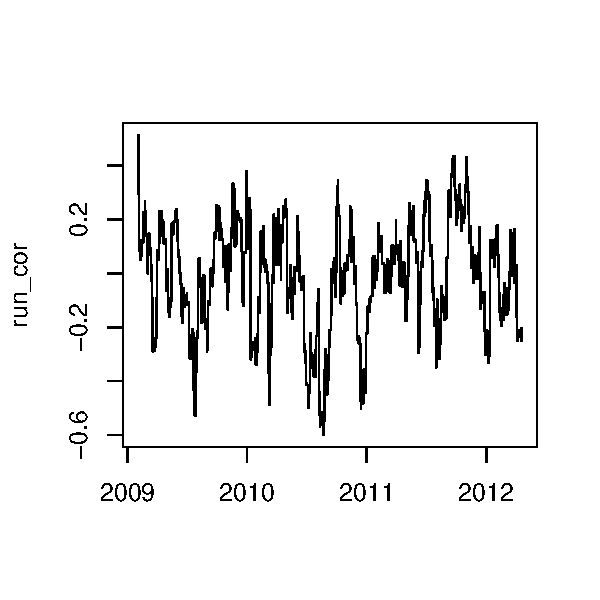
\includegraphics[width=\maxwidth]{figure/unnamed-chunk-18} 

}



\end{knitrout}

Is the running correlation a stationary series?
\begin{knitrout}
\definecolor{shadecolor}{rgb}{0.969, 0.969, 0.969}\color{fgcolor}\begin{kframe}
\begin{alltt}
\hlkwd{require}\hlstd{(tseries)}
\hlkwd{adf.test}\hlstd{(run_cor)}
\end{alltt}


{\ttfamily\noindent\color{warningcolor}{\#\# Warning: p-value smaller than printed p-value}}\begin{verbatim}
## 
## 	Augmented Dickey-Fuller Test
## 
## data:  run_cor
## Dickey-Fuller = -5.38, Lag order = 9, p-value = 0.01
## alternative hypothesis: stationary
\end{verbatim}
\end{kframe}
\end{knitrout}

Can we use a classic ARIMA model to try to predict future correlations? Below we let R automatically search for an ARIMA structure based on Maximum Likelihood. We also plot a series based on the simulated data generated by the "best" model selected as well as its histogram.
\begin{knitrout}
\definecolor{shadecolor}{rgb}{0.969, 0.969, 0.969}\color{fgcolor}\begin{kframe}
\begin{alltt}
\hlkwd{require}\hlstd{(forecast)}
\hlstd{cor.fit} \hlkwb{=} \hlkwd{auto.arima}\hlstd{(run_cor)}
\hlkwd{plot}\hlstd{(}\hlkwd{forecast}\hlstd{(cor.fit,} \hlkwc{h} \hlstd{=} \hlnum{20}\hlstd{))}
\end{alltt}
\end{kframe}

{\centering 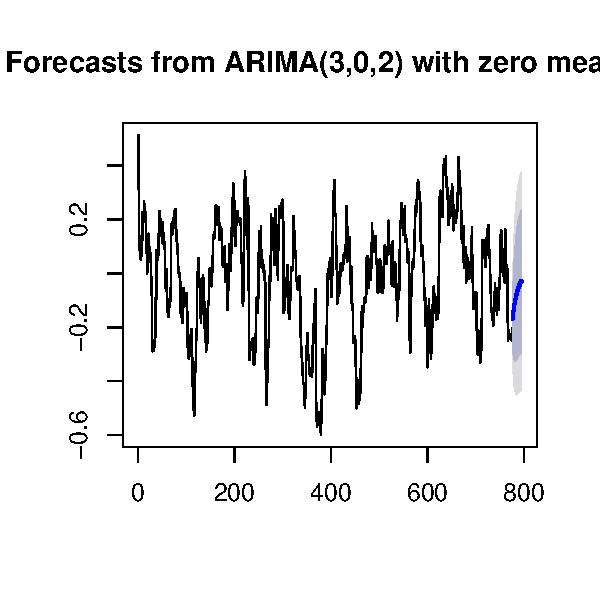
\includegraphics[width=\maxwidth]{figure/unnamed-chunk-201} 

}


\begin{kframe}\begin{alltt}
\hlkwd{set.seed}\hlstd{(}\hlnum{123}\hlstd{)}
\hlkwd{plot}\hlstd{(}\hlkwd{simulate}\hlstd{(cor.fit,} \hlkwc{nsim} \hlstd{=} \hlkwd{length}\hlstd{(run_cor)),} \hlkwc{lwd} \hlstd{=} \hlstr{"2"}\hlstd{,} \hlkwc{col} \hlstd{=} \hlstr{"red"}\hlstd{,} \hlkwc{ylab} \hlstd{=} \hlstr{""}\hlstd{,}
    \hlkwc{xlab} \hlstd{=} \hlstr{""}\hlstd{)}
\end{alltt}
\end{kframe}

{\centering 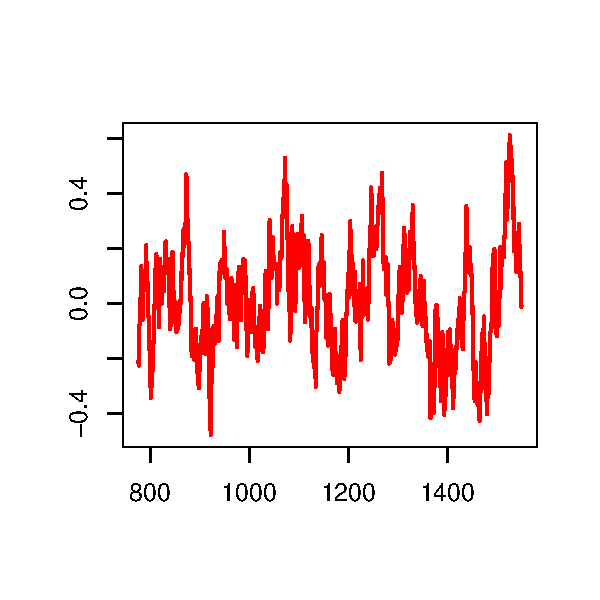
\includegraphics[width=\maxwidth]{figure/unnamed-chunk-202} 

}


\begin{kframe}\begin{alltt}
\hlstd{cor.mat} \hlkwb{=} \hlkwd{matrix}\hlstd{(}\hlkwc{ncol} \hlstd{=} \hlnum{1000}\hlstd{,} \hlkwc{nrow} \hlstd{=} \hlkwd{length}\hlstd{(run_cor))}
\hlkwa{for} \hlstd{(i} \hlkwa{in} \hlnum{1}\hlopt{:}\hlnum{1000}\hlstd{) cor.mat[, i]} \hlkwb{=} \hlkwd{simulate}\hlstd{(cor.fit,} \hlkwc{nsim} \hlstd{=} \hlkwd{length}\hlstd{(run_cor))}
\hlkwd{hist}\hlstd{(cor.mat[}\hlkwd{length}\hlstd{(run_cor), ],} \hlkwc{breaks} \hlstd{=} \hlnum{30}\hlstd{,} \hlkwc{main} \hlstd{=} \hlstr{""}\hlstd{,} \hlkwc{xlab} \hlstd{=} \hlstr{""}\hlstd{)}
\end{alltt}
\end{kframe}

{\centering 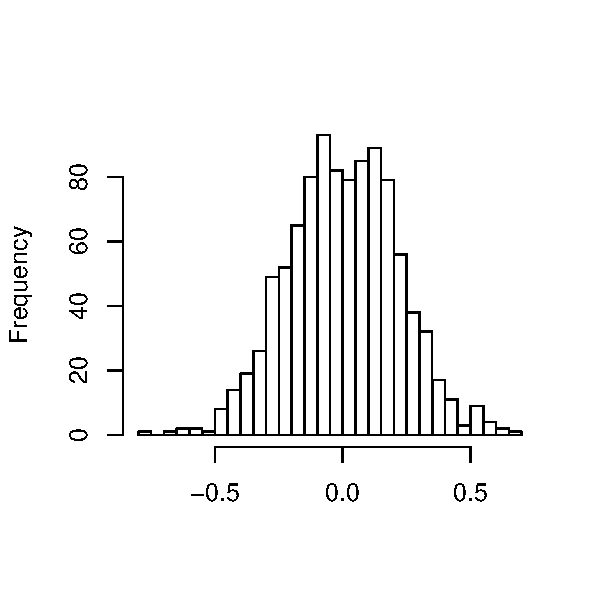
\includegraphics[width=\maxwidth]{figure/unnamed-chunk-203} 

}



\end{knitrout}

As a reference, the summary report of the \textbf{auto.arima} process used to select the "best" model is shown below.
\begin{knitrout}
\definecolor{shadecolor}{rgb}{0.969, 0.969, 0.969}\color{fgcolor}\begin{kframe}
\begin{alltt}
\hlkwd{summary}\hlstd{(cor.fit)}
\end{alltt}
\begin{verbatim}
## Series: run_cor 
## ARIMA(3,0,2) with zero mean     
## 
## Coefficients:
##         ar1    ar2     ar3    ma1     ma2
##       0.587  0.878  -0.533  0.439  -0.521
## s.e.  0.455  0.049   0.386  0.478   0.459
## 
## sigma^2 estimated as 0.00536:  log likelihood=925.2
## AIC=-1838   AICc=-1838   BIC=-1811
## 
## Training set error measures:
##                     ME    RMSE    MAE    MPE  MAPE   MASE      ACF1
## Training set -0.001502 0.07322 0.0516 -70.44 195.1 0.9959 -0.006017
\end{verbatim}
\end{kframe}
\end{knitrout}

\end{document}
